\DocumentMetadata{
  lang = en,
  tagging = on,
  pdfstandard = ua-2
}
%%%%%%%%%%%%%%%%%%%%%%%%%%%%%%%%%%%%%%%%%%%%%%%%%%
%
% LaTeX Template for extended abstracts for the
% ISSW 2026 in Whistler, Canada.  
%  To meet accessibility Requirements this is a completly new template. The .cls file is therefore new and in the .tex file you wil find some slight adaptions of how to handle figures and tables 
% Cheers Machtl 
%
%%%%%%%%%%%%%%%%%%%%%%%%%%%%%%%%%%%%%%%%%%%%%%%%%%
%               * INSTRUCTIONS *
%
%           **** VERY IMPORTANT ****
%
%
%  1 - Rename this file
%  
%  2 - Write your contribution
%
%  3 - Compile with: LuaLaTeX, Biber, LuaLaTeX, LuaLaTeX --> PDF/UA-2-compliant structure
%
%  4 - Follow instructions below and come to Whistler
%%%%%%%%%%%%%%%%%%%%%%%%%%%%%%%%%%%%%%%%%%%%%%%%%%

\documentclass{issw}

\usepackage[base]{babel}
\usepackage{graphicx}
\usepackage{amsmath}
\usepackage{booktabs}
\usepackage{tagpdf}
\tagpdfsetup{
  activate-all            = true,
  math/mathml/luamml/load = true,
  math/alt/use            = true
}

\addbibresource{references.bib}

\usepackage{parskip} % no indent with new paragraph

% Consistent feature-name formatting (matches Table 1 everywhere it's used)
\newcommand{\HS}{\mathrm{HS}}
\newcommand{\HNtf}{\mathrm{HN24}}
\newcommand{\TAmax}{TA_{\mathrm{max}}}
\newcommand{\Snmin}{Sn38_{\mathrm{min}}}
\newcommand{\dlwl}{\texttt{depth\_lower\_wl}}

% ================= TITLE, AUTHOR==================================================
\title{Forecasting Avalanches in Data-Sparse Central Asia Using \\
Snowpack and Weather Modeling with Avalanche Observations}

\author[1]{Itai Sheleg\corref{complete\_address}}
\author[2]{Doug Chabot}
\author[3]{John Snook}
\author[1]{Jaime Peters}
\author[4]{Walter Steinkogler}
\author[3]{Ron Simenhois}



\address[1]{Lake County High School, Leadville, CO, USA}
\address[2]{Latok, LLC, Bozeman, MT, USA}
\address[3]{Colorado Avalanche Information Center, CO, USA}
\address[4]{Wyssen Avalanche Control AG, Switzerland}

\cortext[complete\_address]{
Itai Sheleg, Lake County High School, \\
Leadville, CO, USA,\\
email: itai.sheleg@gmail.com}
% ===================================================================

\begin{document}

% ==================== ABSTRACT ===============================================
\begin{abstract}
Avalanches in Central Asia, particularly in Afghanistan, Tajikistan, and Pakistan, are a persistent hazard, causing hundreds of fatalities in severe winters and routinely destroying homes, infrastructure, and livestock essential for survival. To address this risk, in 2015, Aga Khan Agency for Habitat established a remote avalanche forecasting program supported by external expertise.
Following its implementation, it became clear that a primary constraint on forecasting capability is the limited availability of snowpack, weather, and avalanche observations, driven by both geographic remoteness and government restrictions on data sharing.
We address this gap by developing a proof-of-concept framework that fuses heterogeneous, publicly available data sources to support avalanche forecasting in data-sparse regions. Specifically, we combine numerical weather prediction (NWP)-forced SNOWPACK simulations (4 km grid spacing) with opportunistically extracted avalanche observations from social media posts shared by local residents. This approach treats informal reports as weakly labeled observations, enabling the reconstruction of avalanche occurrence in the absence of systematic records.
We compiled 69 valley-floor avalanche observations from social media and AKAH field logs across two winters, and matched each to the nearest SNOWPACK station sharing its predominant aspect, reconstructing the associated meteorological and snowpack conditions at 30 virtual stations. Five daily variables drive the model: total snow depth, 24-hour new snow, maximum air temperature ($\TAmax$), the whole-profile minimum natural stability index ($Sn38$), and the burial depth of the weakest layer. To distinguish avalanche from non-avalanche days, we fit a hierarchical Bayesian logistic regression that gives each station its own baseline avalanche rate while sharing the influence of the five variables across the network.
Trained on 2024–2025 and evaluated on the unseen 2025–2026 season, the model ranks avalanche days above quiet ones with an AUC-ROC of 0.715 and an average precision 7.0 times the no-skill baseline. Total snow depth carries the most weight, followed by weak-layer burial depth, which lowers risk as it deepens. New snow and $\TAmax$ both raise risk, with warming weighing about as much as new-snow loading, suggesting that warm, likely rain-influenced storms are at least as important as loading in driving these events. Detection improves steeply with local history, from 56\% with one prior logged event at a station to 100\% with three, and four stations already meet an operational false-alarm standard of roughly one per month.
This work incorporates a novel data-fusion and weak-supervision framework for avalanche forecasting, integrating NWP-driven snowpack modeling with opportunistic, publicly sourced observations. However, this framework is constrained by a limited event dataset and a model chain that lacks rigorous, component-wise validation, introducing uncertainty in both inputs and predictions. As such, the framework is best interpreted as a decision-support tool rather than a fully autonomous forecasting system. Coupled with expert validation and interpretation, it provides a scalable pathway for developing operational guidance in regions where conventional data streams are sparse or unavailable.
\end{abstract}

\begin{keyword}
Avalanche Forecasting, SNOWPACK, Bayesian Modeling, Central Asia
\end{keyword}

\maketitle
% ===================================================================


\section{INTRODUCTION}
Avalanches are a severe and recurring hazard across the Hindu Kush, Pamir, Karakoram, and western Himalaya. A single 2012 avalanche cycle in Afghanistan, Pakistan, and Tajikistan killed more than 100 people \parencite{ChabotKaba2016}, motivating the Aga Khan Development Network and Aga Khan Agency for Habitat (AKAH) to build a community-based avalanche warning system around village-run weather monitoring posts, coordinated evacuation planning, and trained search-and-rescue teams. When a comparably severe cycle struck the same region in February 2023, 38 people died \parencite{Chabot2024}, a fraction of the 2012 toll attributed to the network built in the intervening years. Providing operational avalanche forecasts is a central component of these programs, yet the observational data that underpin modern forecasting are largely unavailable across the region.
Modern avalanche forecasting relies on dense observational networks, including automated weather stations, snowpack observations, and systematic avalanche records. Across much of Central Asia, this infrastructure is largely absent, and the challenge has three components. Field snowpack observations are essentially absent. Automated weather stations are rare at avalanche-relevant elevations, and where they exist, cost constraints and government restrictions on cross-border data sharing often prevent their use in regional forecasting \parencite{Chabot2024}. Systematic records of avalanche occurrence needed to establish historical baselines and evaluate model performance are similarly lacking. Each limitation would significantly constrain an operational forecasting program; together, they render conventional forecasting approaches impractical.
We combine three globally available data sources: numerical weather prediction (NWP) model output, satellite imagery, and avalanche events identified from social media and local news reports to test whether these limitations can be substantially mitigated. Systematic records of avalanche events in this region exist almost entirely outside peer-reviewed literature, in technical reports, news, and social media \parencite{Acharya2023}, making these sources not merely supplementary but the primary available record. This paper focuses on the NWP-driven snowpack modeling and observation components of the framework; satellite-derived inputs are part of the broader system architecture but fall outside the present evaluation.
This paper presents the system architecture and a pilot deployment in Afghanistan, Pakistan, and Tajikistan. The operational network runs 1155 virtual SNOWPACK stations; the evaluation reported here uses the 30 stations matched to 69 avalanche observations compiled from AKAH's structured observation logs and social media reports. We evaluate how well the model separates avalanche days from quiet ones, whether that skill holds up in a season it has never seen, and whether the weights it learns are physically coherent, then discuss the steps required to transition the framework toward reliable operational forecasting in data-sparse regions worldwide.

\section{DATA}
\subsection{NWP Forcing and SNOWPACK Simulations}
We implemented the Weather Research and Forecasting model (WRF) \parencite{SkamarockKlemp2008} over Central Asia in 2022 to produce winter weather forecasts. Initial and lateral boundary conditions come from the US National Weather Service Global Forecast System (GFS). We run a nested grid, a 12-km outer domain with a 4-km inner nest, and put out 7-day forecasts twice a day. Post-processing turns that into standard parameter imagery and point forecasts on a regional website. The first winter told us the forecasts were worth building on.
The following season we added SNOWPACK \parencite{Lehning2002,Morin2020}, following the approach the Colorado Avalanche Information Center developed \parencite{SnookEtAl2022,Snook2016}. WRF writes meteorological output straight into SNOWPACK, which simulates layer-by-layer snowpack evolution at each grid point. The system builds profiles at every 4-km grid point above 3,500 m inside the forecast domain, updates them daily, and serves them on the same website, with full seasonal profiles available on demand.
For this study, we pulled SNOWPACK output from 30 virtual stations that turned out to be nearest to at least one avalanche report across the Darvoz district of Tajikistan and northwest Pakistan. Each station carries a specific aspect (N, E, S, W, or flat) and elevation, so the network represents snowpack evolution tuned to slope exposure rather than one regional average. We ran two consecutive winters: 2024–2025 for training, 2025–2026 for evaluation. Sub-daily {\texttt{.smet}} files gave us the meteorological time series, and {\texttt{.pro}} files gave us per-layer stratigraphy at each timestep. Table \ref{tab:table_1} lists the five variables the model uses. Figure \ref{fig:study_area_map} shows the station network and a representative forecast window from 2025–2026.

\begin{table*}[t]
  \centering
  \caption{The five model features, their SNOWPACK source, and physical role.}
  \label{tab:table_1}
  \begin{tabular}{lll}
    \hline
    \textbf{\textit{Feature}} & \textbf{\textit{Source}} & \textbf{\textit{Physical role}} \\
    \hline
    $\HS$ & SNOWPACK & Total snow depth: size / valley-reach potential \\
    $\HNtf$ & NWP & 24-hour new snow: primary loading trigger \\
    $\TAmax$ & NWP & Daily max air temperature: wet vs dry mechanism \\
    $\Snmin$ & SNOWPACK & Whole-profile minimum stability index: weakest-layer strength \\
    \dlwl & SNOWPACK & Weak-layer depth: proximity to ground / basal layer \\
    \hline
  \end{tabular}
\end{table*}

\begin{figure*}[ht]
  \centering
  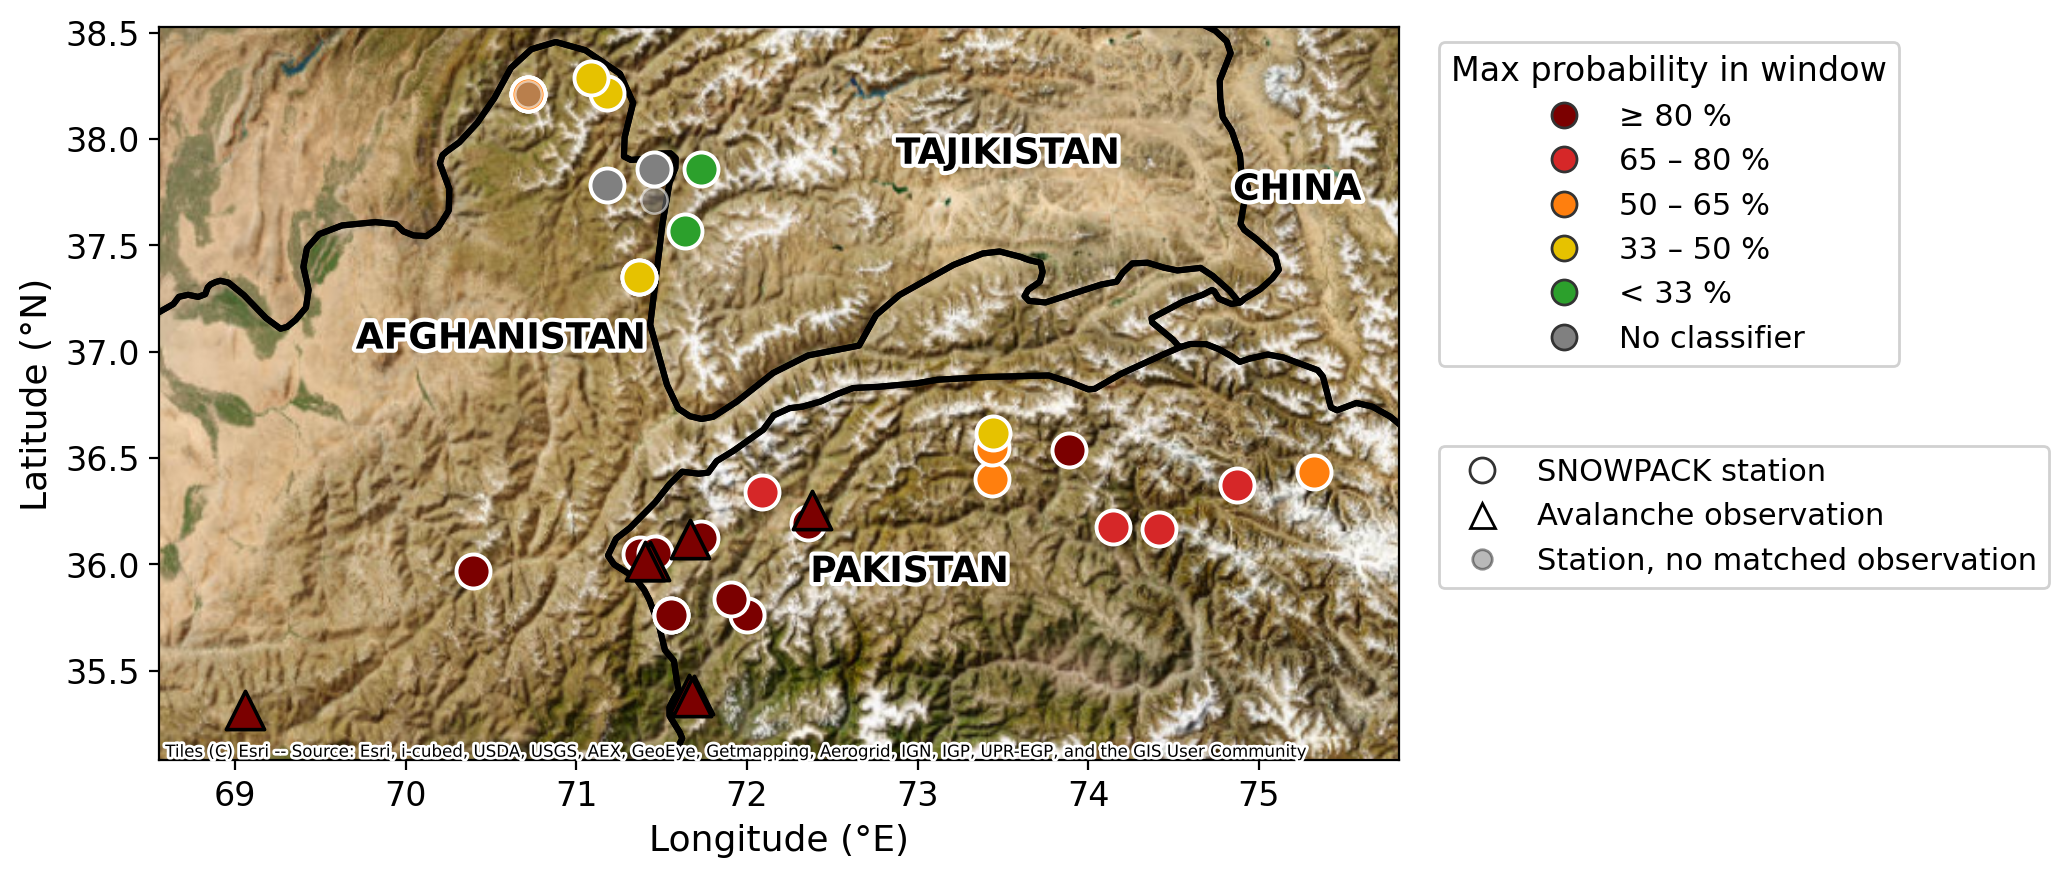
\includegraphics[
    width=0.85\textwidth,
    alt={Satellite image of the study area spanning Tajikistan, northeast Afghanistan, and northwest Pakistan. Circles are SNOWPACK virtual stations colored by modeled probability for the January 22-25, 2026 forecast window, from green (low) through gold and orange to dark red (at least 80 percent); triangles mark the eight avalanche reports from January 23, 2026, colored the same way. A cluster of dark-red stations and triangles appears in the southern group, coinciding with most of the reported events.}
  ]{./figures/fig1_map.png}
  \caption{Study area map with the January 23, 2026 event cycle selected. Triangles mark the valley-floor avalanche reports for that date; circles are SNOWPACK virtual stations with rings colored by modeled probability in the January 22–25 forecast window. The dark-red cluster ($\geq$80\%) coincides with the reported events, while stations without matching observations are shown faded.}
  \label{fig:study_area_map}
\end{figure*}

\subsection{Avalanche Observations}
AKAH collects avalanche reports and forwards them to the forecaster. Almost all of them come from locals' Facebook pages in Afghanistan and Pakistan, and off Instagram in Tajikistan. Most carry video or photographs showing how far the avalanche ran, which is more than we get from most formal reporting channels in the region.

\begin{figure}[ht]
  \centering
  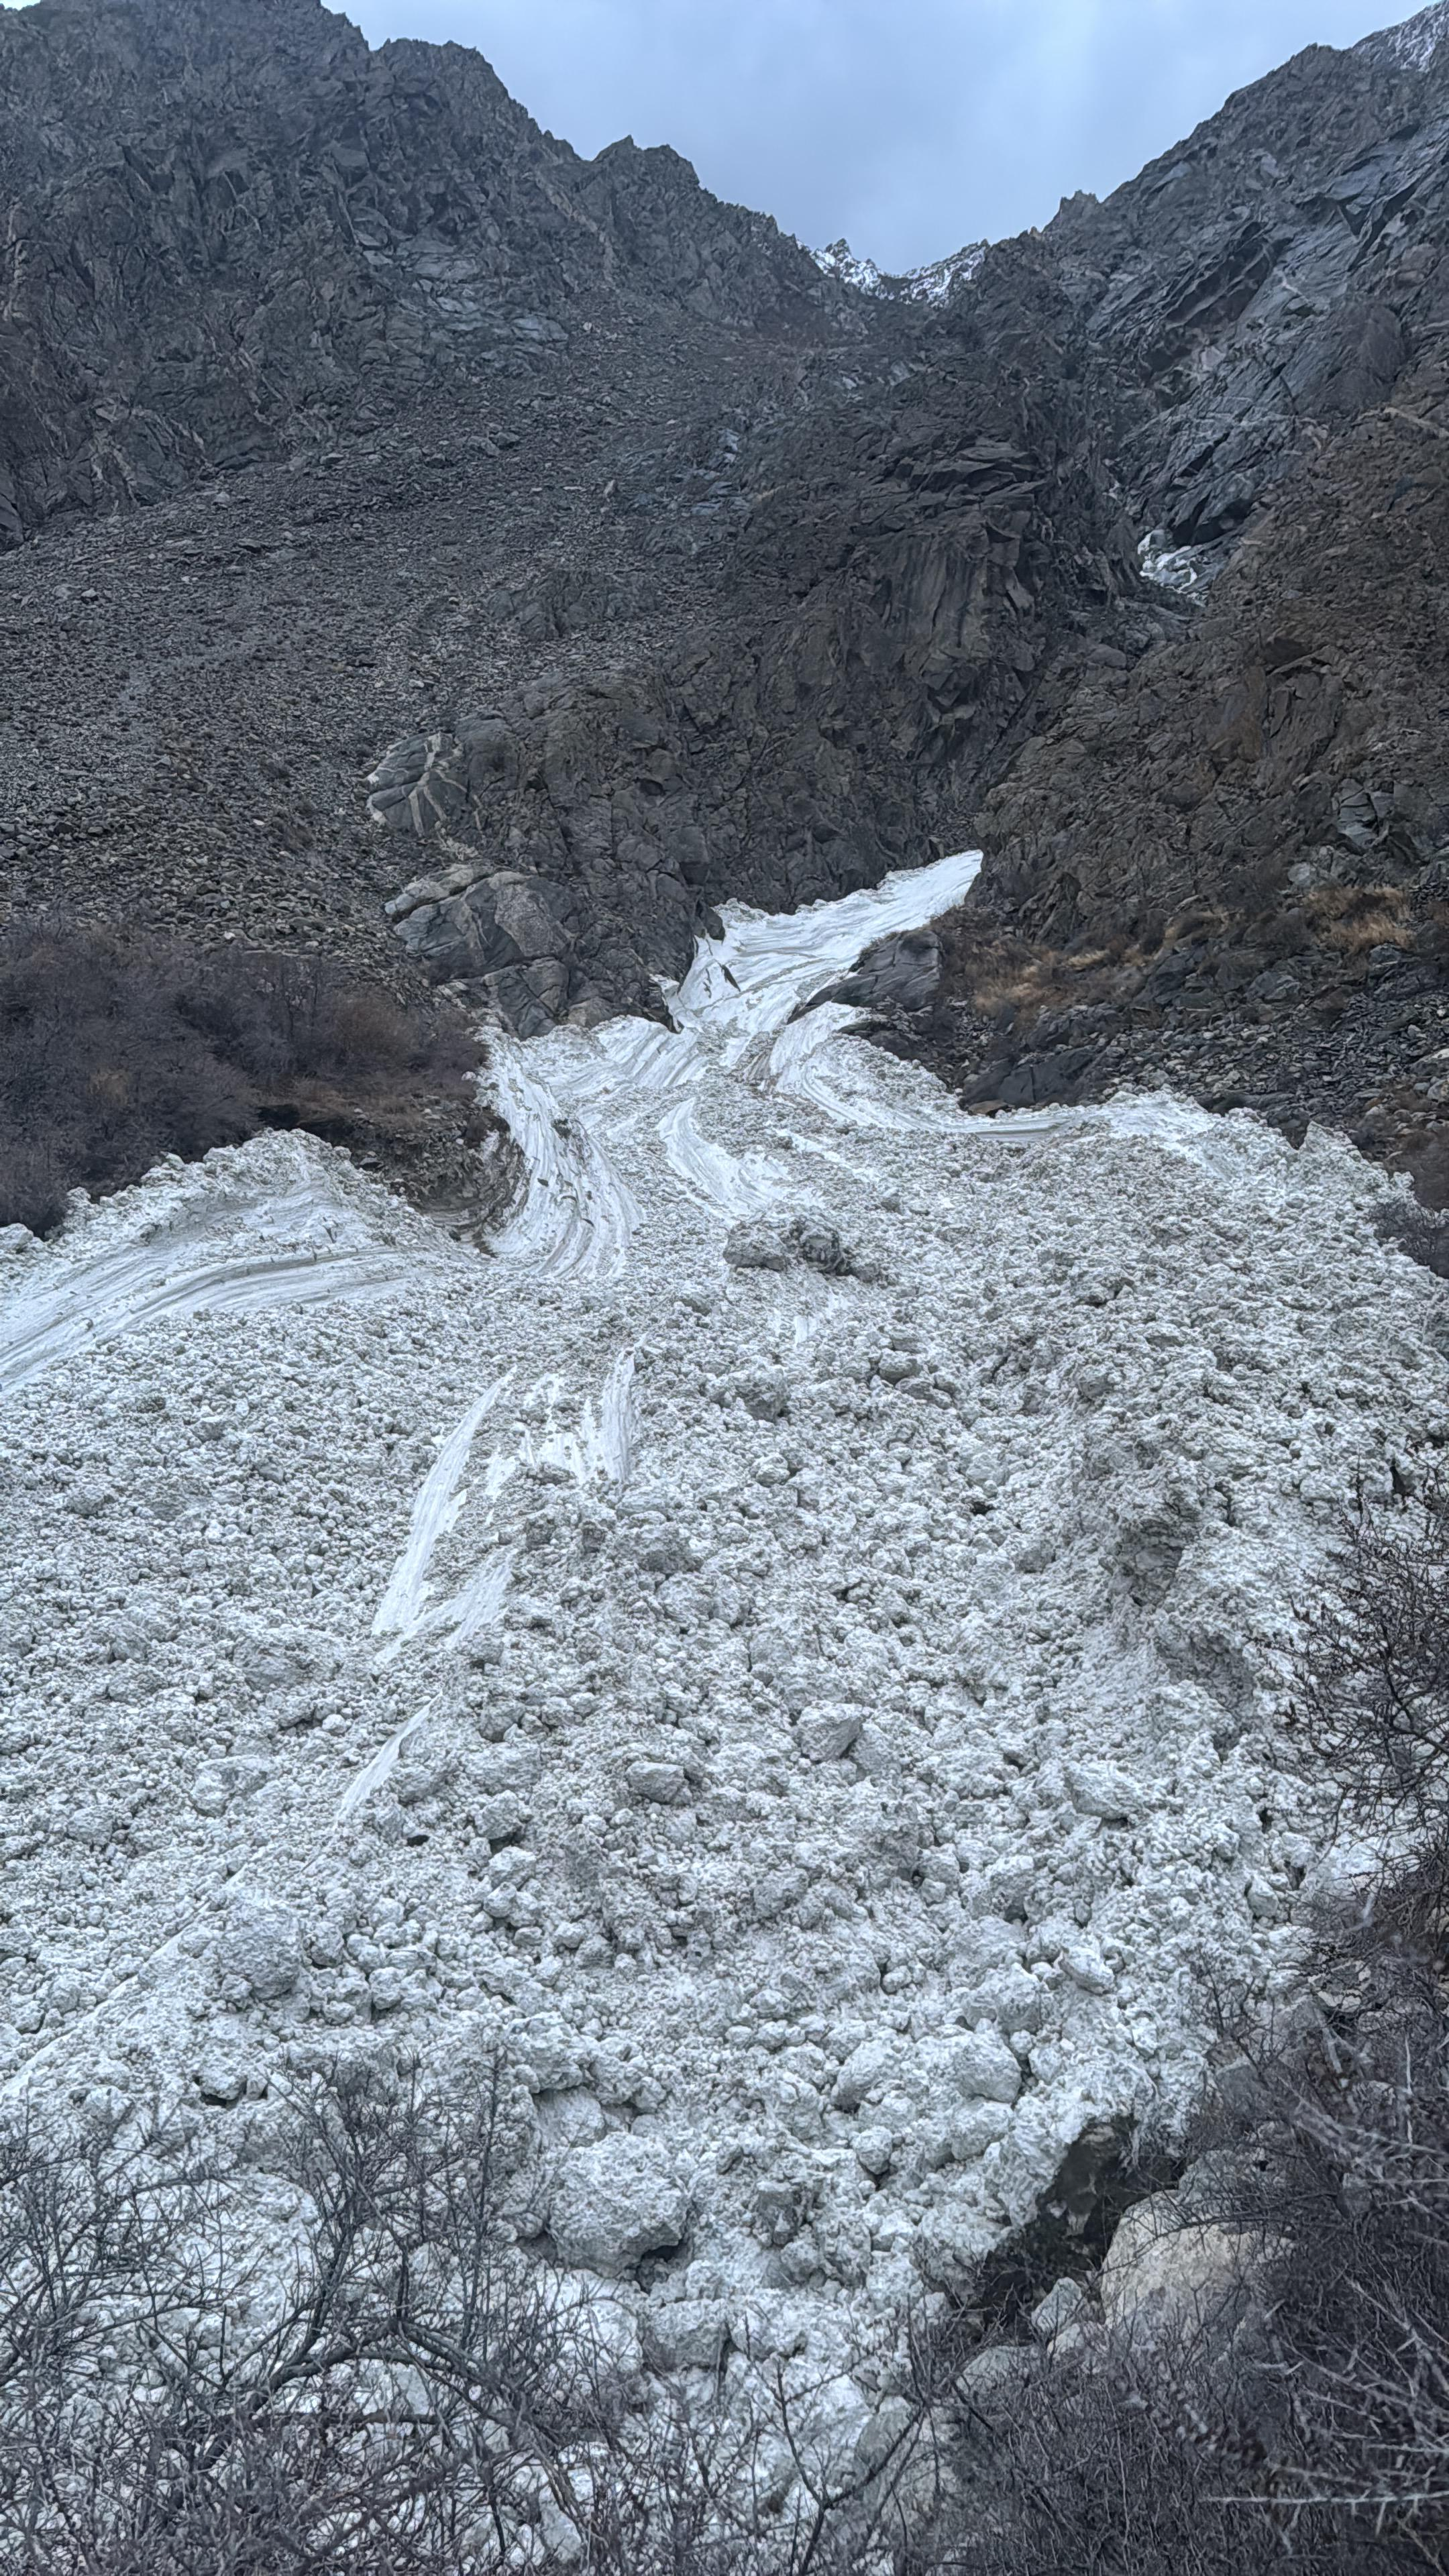
\includegraphics[
    width=0.8\columnwidth,
    alt={Ground-level photograph of avalanche debris filling a narrow rocky gully, taken looking up-path. Chunky white debris blocks cover the gully floor and lower banks in the foreground; bare rock walls converge toward a notch at the skyline, and no start zone is visible from this vantage.}
  ]{./figures/fig1b_observation_photo.jpg}
  \caption{A valley-floor avalanche photo of the kind local observers post to Facebook and Instagram and AKAH compiles into the observation dataset. The debris is visible, but the start zone is not. This is the gap this paper's start-zone matching (Section \ref{sec:obs-matching}) is built to close.}
  \label{fig:observation_example}
\end{figure}

These posts give valley-floor runout locations, not start zones. Each has a date, an approximate location, and rough estimates of slope angle, aspect, and size, derived from the posts rather than measured. AKAH provided the initial notification of avalanche events, but every piece of observational data used here was pulled independently from publicly available posts. The combined set holds 69 observations: 26 from 2024–2025 and 43 from 2025–2026.
We treat these as weakly labeled events. A post confirms that an avalanche reached the valley floor. It says nothing about the trigger, the release zone, or the state of the snowpack. More importantly, no post does not mean no avalanche. Our record is opportunistic and almost certainly incomplete, so some unknown number of real events sit in the data as quiet days.
That is a positive-unlabeled problem \parencite{ElkanNoto2008}, and the practical consequence works in our favor. Any skill we report is a conservative floor, because some of the quiet days the model gets penalized for flagging probably did have avalanches nobody posted about. The supplementary technical report \parencite{ShelegEtAl2026} covers this in more detail, including why we apply no formal correction for it.

\subsection{Observation-to-Station Matching}
\label{sec:obs-matching}
Valley-floor reports provide approximate runout locations rather than start zones. For each observation, the forecaster, who has regional terrain knowledge, worked out the likely start zone from valley geometry, known paths, and whatever context came with the report. We then matched each start zone to the nearest SNOWPACK station sharing the same predominant aspect (N, E, S, or W), so the simulation reflects the right solar radiation and wind loading regime.
That hybrid step puts terrain knowledge where distance alone would fail. Two stations equidistant from a reported runout but facing opposite aspects can carry completely different snowpack histories. This matching introduces forecaster subjectivity and is not automatically reproducible. We consider that a feature rather than a gap. It is the mechanism through which terrain expertise enters the framework.

\section{METHODS}
\subsection{Feature Engineering}
We aggregated sub-daily SNOWPACK output to one value per day. From the weather side we took daily maxima for total snow depth ($\HS$), 24-hour new snow ($\HNtf$), and air temperature ($\TAmax$). From the modeled profile, we split each timestep into an upper zone, everything buried shallower than 40\% of total depth, and a lower zone below. The upper zone is where storm slabs live; the lower zone is where persistent weak layers sit. Within each zone we took the minimum ${Sn38}$ stability index, plus the burial depth of the weakest layer in the lower zone.
The 2024–2025 training set holds 35 positive days across the 13 stations with usable 2024–2025 SNOWPACK data. Anything larger would be modeling noise instead of signal. The five variables in Table \ref{tab:table_1}: $\HS$, $\HNtf$, $\TAmax$, $\Snmin$, and \dlwl\ are physically distinct and do not track each other closely.

\subsection{Labeling Under Weak Supervision}
An event day gets labeled positive, and so does the day before it, accounting for the one-day reporting lag inherent in social media and field log sources. Every other day is negative. That leaves roughly 0.7\% of days positive in the 2024–2025 training set, an imbalance worth remembering when reading the skill scores.
Some stations had no valid zone features on positive days, usually early season with little snow down. Those fell back to weather alone ($\HS$, $\HNtf$, $\TAmax$), sacrificing snowpack structural information but preserving trainability.

\subsection{Combining Station and Regional Data}
We built one model that lets every station borrow from the rest of the region while keeping its own local signal \parencite{GelmanHill2007}. Each of the 13 stations with at least one recorded event holds its own baseline avalanche rate. The influence of the five variables is shared across the whole network.
How much a station leans on itself versus the region is learned from the data, not set by us. A station with several observed events keeps mostly its own signal. A station with one event leans heavily on the regional average. That is the behavior you want from a sparse network: trust local history where there is enough of it, fall back on regional experience where there is not.
We left stations with no recorded events out of training. In this region, an empty record more likely means nobody was watching than that nothing ran, and training on the opposite assumption teaches the model the wrong lesson. At prediction time, those stations are served by the regional pattern.
This also gives us a confidence estimate on every prediction at no extra cost, which Section \ref{sec:model-uncertainty} describes. The model is a hierarchical, or multilevel, logistic regression, fit with PyMC \parencite{AbrilPla2023}.

\subsection{Evaluation}
We tested the model three ways:
\begin{enumerate}
  \item \textbf{Rolling per-station test.} For each station, we put its observed events in time order and asked whether the model warned before each one, using only what it knew beforehand. Each test trains on everything that came earlier at that station, pulling from either season, and tests on the next event. Training only looks backward, so no future information leaks in. This measures how much accumulated local history helps. It mixes seasons on purpose, so it is not a test of a brand-new year. We counted an event as detected if the highest predicted probability in the three days up to and including the event reached 50\%.
  \item \textbf{Cross-season holdout.} We trained on 2024–2025 only and evaluated entirely on 2025–2026, so nothing from the test season ever reached training. This is the honest test of whether the model holds up in a year it has never seen. We report two scores. AUC-ROC measures how well the model ranks dangerous days above quiet ones, where 1.0 is perfect, and 0.5 is a coin flip. Average precision is the more useful of the two when real events are rare, and they are: about 2\% of station-days carry a positive label in the 2025–2026 evaluation season, versus 0.7\% in 2024–2025 training. That gap is season coverage, not a change in reporting; avalanches were recorded at all 30 matched stations in 2025–2026 but only 15 of 30 in 2024–2025, so more of the pooled 2025–2026 days sit near a reported event \parencite{SaitoRehmsmeier2015}.
  \item \textbf{Event-level scoring.} For each test event, we took the model's highest probability in the three days before it as the warning score, then compared that against equal-length windows on quiet days at the same stations. This asks the question a forecaster cares about, whether a timely warning went out, rather than whether every single day got labeled correctly.
\end{enumerate}

\section{RESULTS}
\subsection{Per-Station Performance and Learning Curve}
We asked the practical question at each station: using only what the model knew before an avalanche ran, did it flag the day? Sixteen stations had enough history to test. Eight caught every event. Three caught about half. Five missed completely, and all five had exactly one prior event to learn from.
The pattern inside that failure is the most useful thing we found (Table \ref{tab:table_2} and Figure \ref{fig:learning_curve}). With one logged event at a station, the model caught 56\% of the next ones. With two, 86\%. With three, it caught all of them. Every added observation delivers a large, consistent gain, and the dataset sits on the steep part of that curve. The limiting factor here is not the model but the number of recorded avalanches. Three events at a station is roughly where we would start trusting it. Detection is only half the ledger: false alarms at a fixed threshold do not improve along the same curve, and the full accounting (threshold sweeps and per-station false alarm rates) is in the supplementary technical report \parencite{ShelegEtAl2026}.

\begin{figure}[ht]
  \centering
  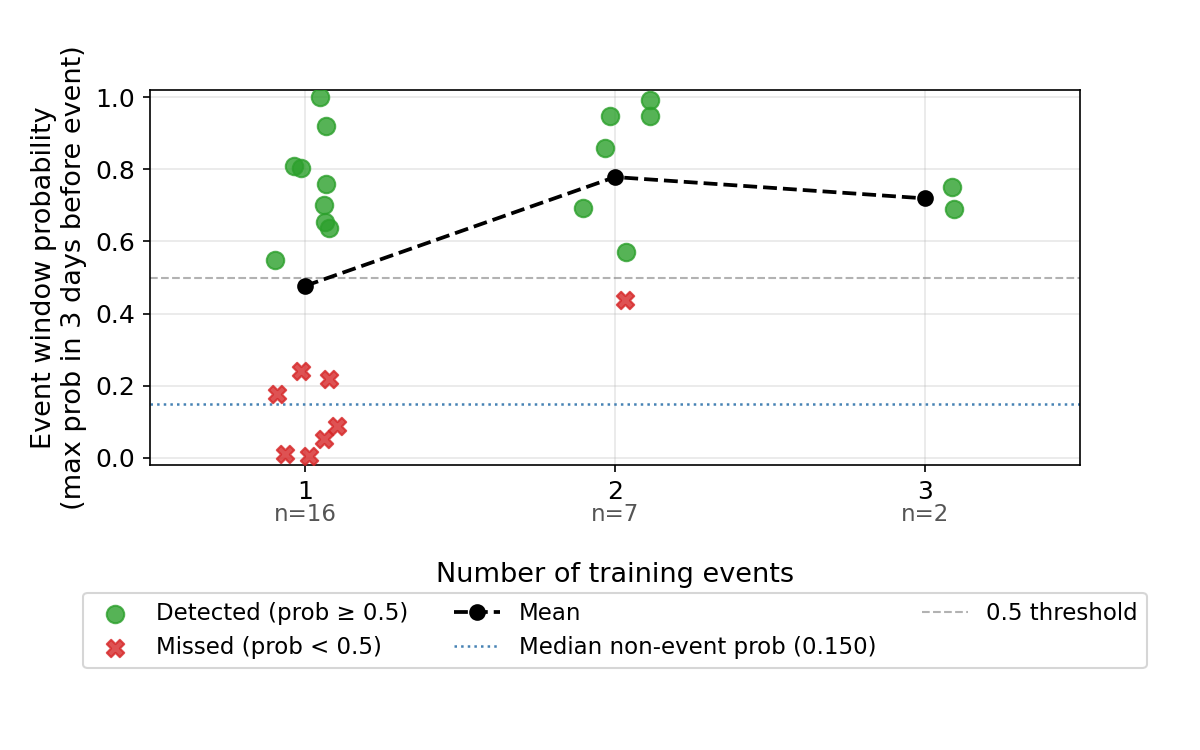
\includegraphics[
    width=1.\columnwidth,
    alt={Scatter plot of per-station event-window probability against number of prior training events. Detected events are green circles and missed events are red X marks, so the two classes are distinguishable by both color and shape; a black dashed mean line rises from 0.48 at one prior event to 0.78 at two and 0.72 at three.}
  ]{./figures/fig2_learning_curve.png}
  \caption{Learning curve: detection rate and mean warning probability as a function of the number of prior observed events at a station.}
  \label{fig:learning_curve}
\end{figure}

\begin{table*}[t]
  \centering
  \caption{Detection rate improves steeply with each additional observed event.}
  \label{tab:table_2}
  \begin{tabular}{lll}
    \hline
    \textbf{\textit{Prior events at station}} & \textbf{\textit{Detection rate}} & \textbf{\textit{Mean warning probability}} \\
    \hline
    1 & 56\% & 0.48 \\
    2 & 86\% & 0.78 \\
    3 & 100\% & 0.72 \\
    \hline
  \end{tabular}
\end{table*}

\subsection{Cross-Season Performance}
The harder test is whether the model holds up in a season it has never seen. We trained on 2024–2025 and evaluated on the 2025–2026 season's 37 unique station-day events (43 raw reports that season, six of which shared a station and date with another report and so collapsed into one event), with nothing from that winter in the training data. It ranked dangerous days above quiet ones with an AUC-ROC of 0.715, and its warnings landed about seven times more precisely than random guessing.
We also tried simpler setups: one model per station, one model for the whole region, and a blend of the two. The shared, hierarchical model beat all of them. A station with few logged events borrows the pattern from better-observed stations nearby while still keeping whatever local history it has. The full model comparison and statistical detail are available in the supplementary technical report \parencite{ShelegEtAl2026}.

\subsection{What the Model Learned}
The weights the model settled on are foundational rules every forecaster already knows (Figure \ref{fig:feature_importance}). Total snow depth dominates: a deep snowpack carries the volume and energy needed to reach the valley floor, and thin years do not produce these events.
Weak-layer burial depth comes second and pulls the other way. The deeper a weak layer sits, the harder it is to trigger, so shallow weak layers drive the modeled risk up.
New snow and warm temperatures both raise risk, and warming carries about as much weight as loading. The ${Sn38}$ stability index adds a smaller, secondary signal. These patterns hold across the region and align with what experienced forecasters expect from the terrain and climate in Central Asia.

\begin{figure}[ht]
  \centering
  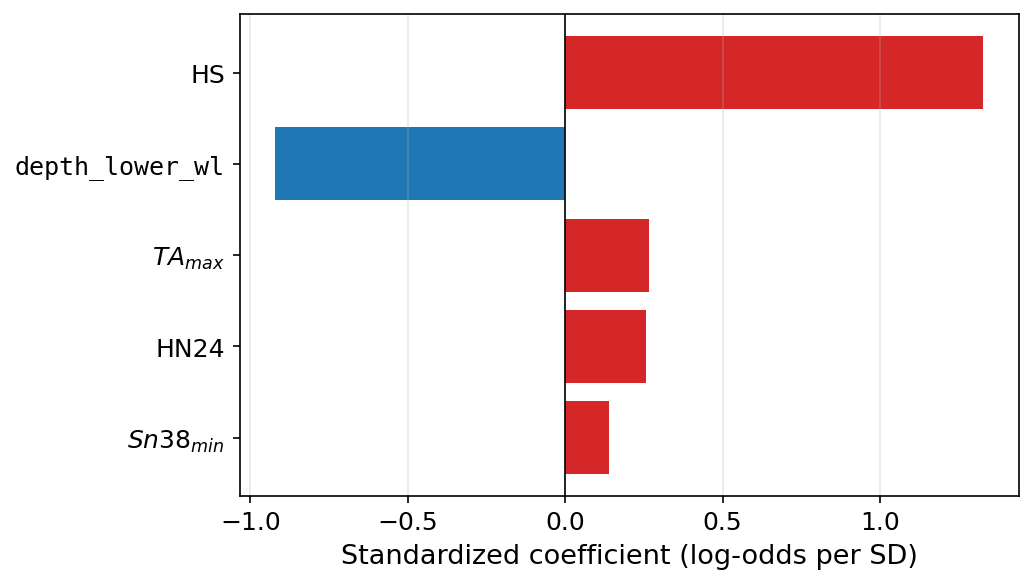
\includegraphics[
    width=1.\columnwidth,
    alt={Horizontal bar chart of standardized logistic-regression coefficients for the five model features. HS has the longest red (risk-increasing) bar, followed by TA_max and HN24; sn38_min is a short red bar; depth_lower_wl is the only blue (risk-decreasing) bar.}
  ]{./figures/fig3_feature_importance.png}
  \caption{Feature influence on predicted avalanche risk, with standardized model coefficients as a horizontal bar chart. Red bars increase risk; blue bars decrease risk; longer bars mean stronger influence.}
  \label{fig:feature_importance}
\end{figure}

\subsection{Knowing What the Model Doesn't Know}
\label{sec:model-uncertainty}
A key advantage of the shared, hierarchical approach is that it reports not just a probability, but how confident it is in that probability. Where a station has several logged events, the estimate is tight. Where it has none, the model falls back on the regional average and flags uncertainty in the prediction.
A high probability at a station with history behind it is a strong signal with confidence. The same number at a station with nothing behind it is a reason to prompt extra caution and expert judgment rather than automated action.

\subsection{Operational Readiness}
We set the bar at roughly one false alarm a month, no more than 10\% of non-event days, since a forecast nobody believes is worse than no forecast at all. Four stations are operationally ready today. One threw zero false alarms across the entire 2025–2026 season; two more flagged fewer than three days all winter.
Three stations sit in a marginal band. Those are usable if a forecaster reviews every alert before it goes out, which is what we currently do.
The rest are not ready, almost always because they have too few logged events to set a threshold on. Another season of reports will move stations from not-ready to marginal or ready.

\subsection{Case Study: Model Output for a Known Event}

\begin{figure*}[ht]
  \centering
  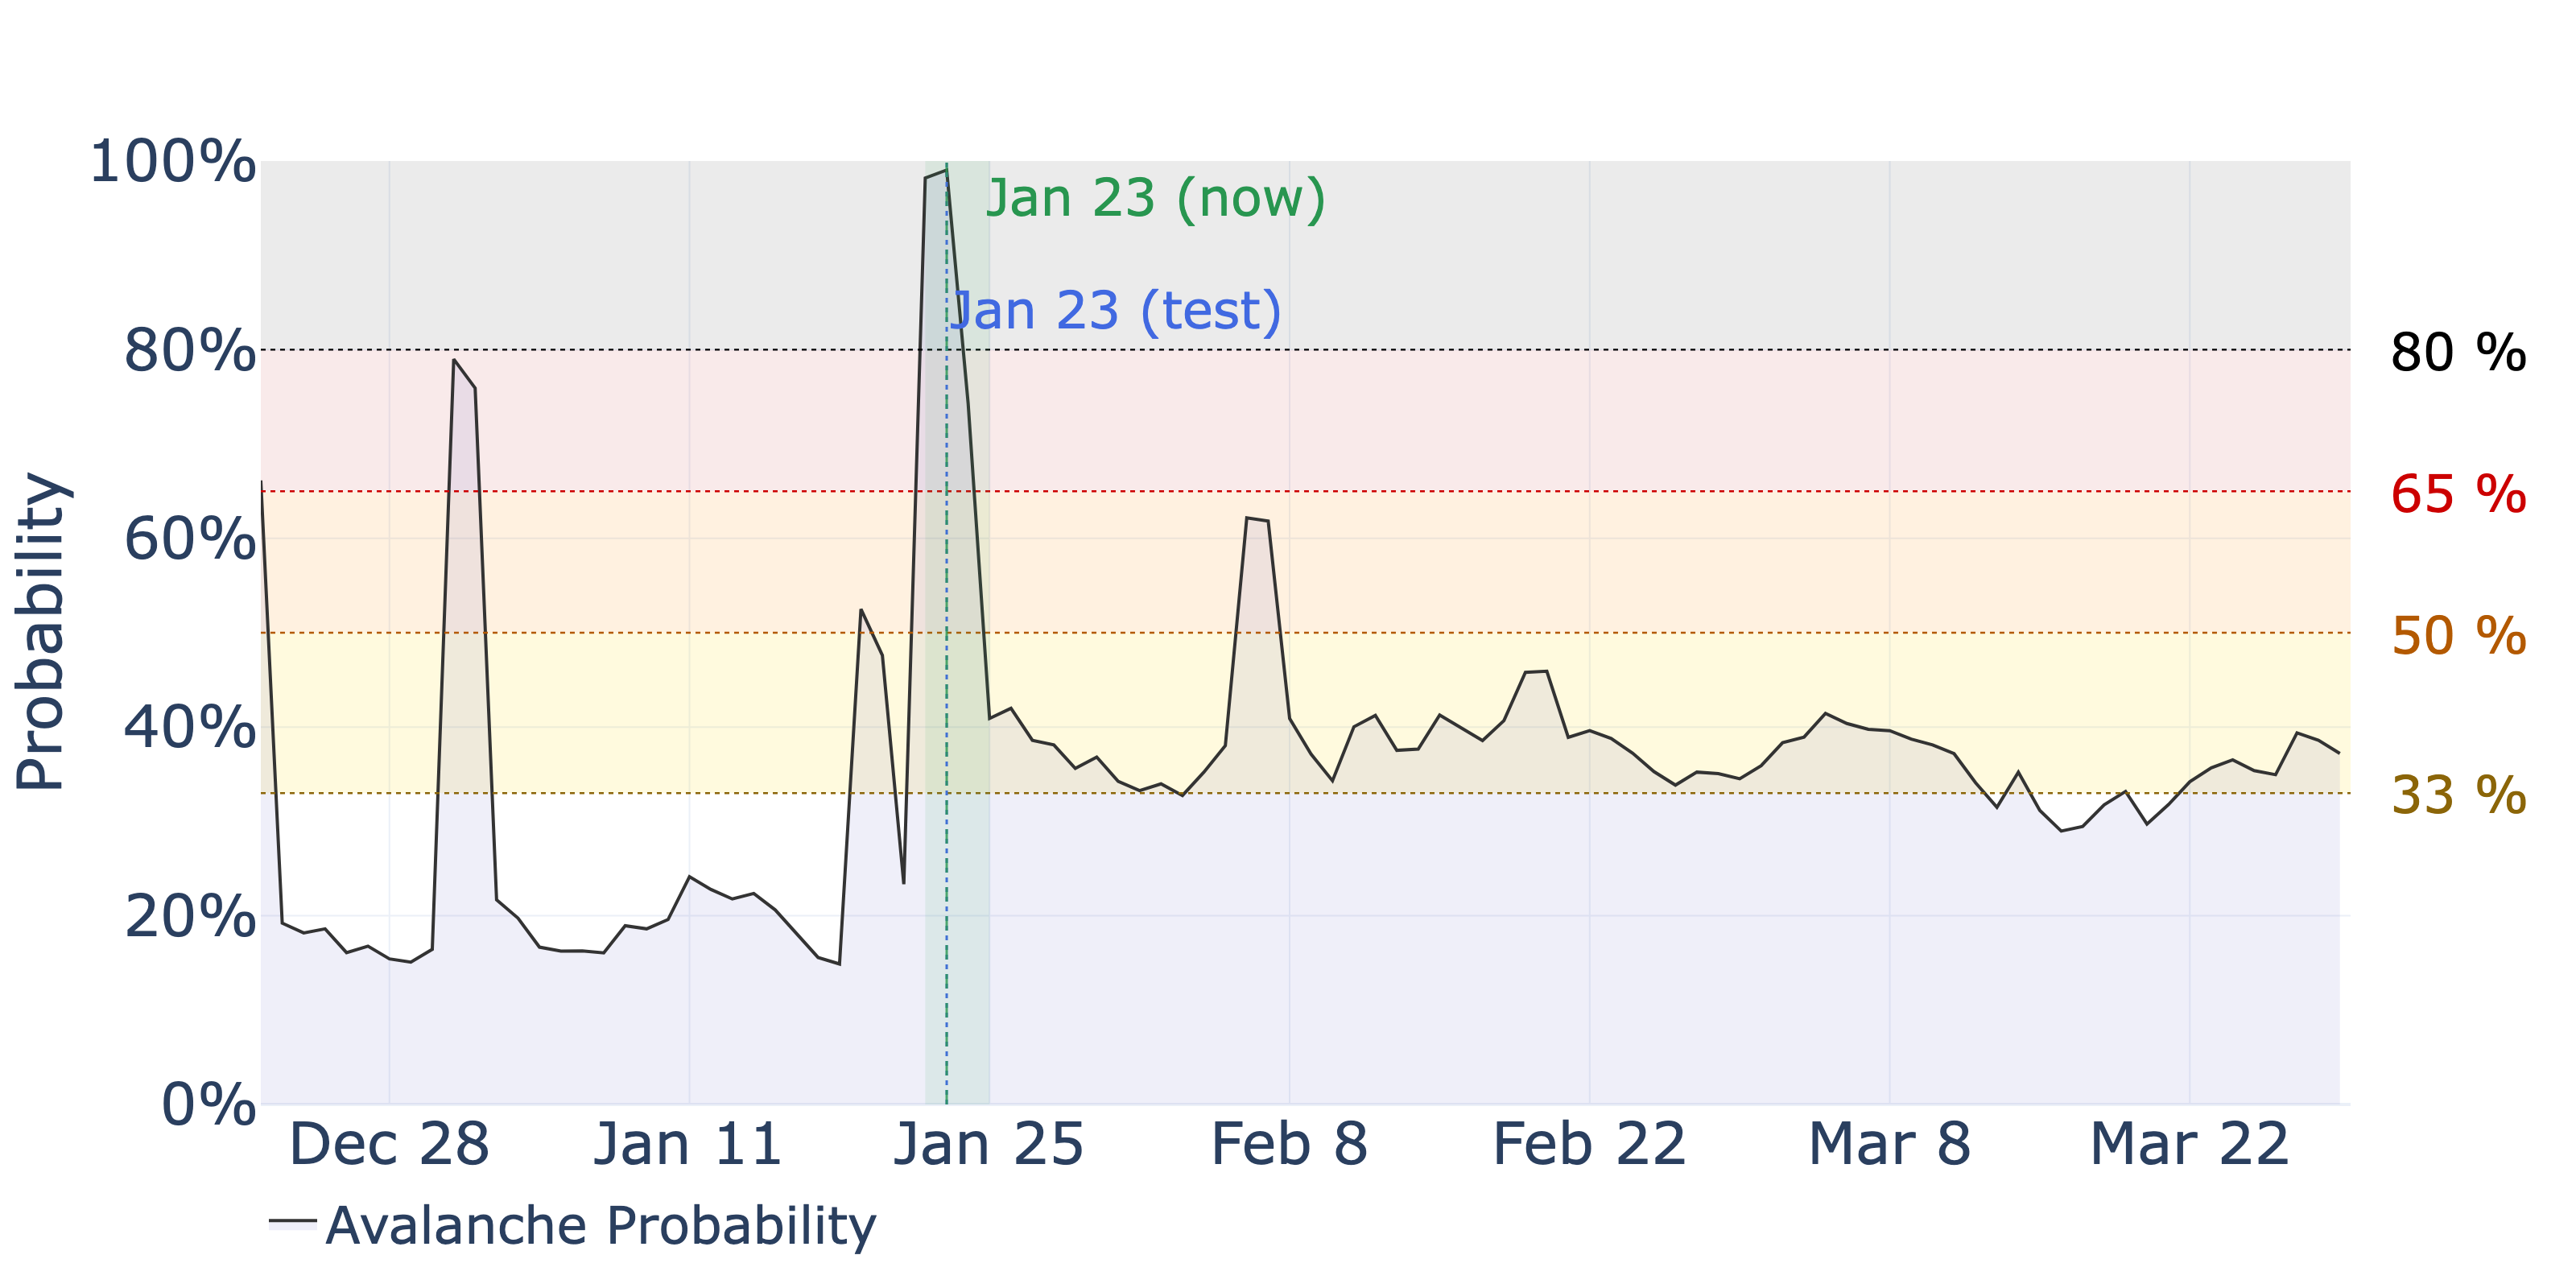
\includegraphics[
    width=0.75\textwidth,
    alt={Avalanche probability chart for station 160942 (east-facing) over the 2025-26 season, with operational threshold bands. Probability peaks near 1.00 in the highlighted three-day window around the January 23 event, and stays well below the 33 percent threshold on most other days.}
  ]{./figures/fig4_stability_160942.png}
  \caption{Per-station avalanche probability for station 160942\_res (east-facing, best-performing station) over the 2025–2026 season, with operational threshold bands. The model assigns probability $\sim$1.00 in the highlighted three-day window around the observed January 23 event, with markedly lower probabilities on surrounding non-event days.}
  \label{fig:case_study}
\end{figure*}

Figure \ref{fig:case_study} shows the best station through the 2025–2026 season. The probability spikes right before the January 23 avalanche cycle, then drops back within days. A narrow, time-specific signal like this is something a forecaster can act on, versus a persistent high-risk background that gets ignored. This chart is what field staff and forecasters actually look at.

\section{DISCUSSION}
\subsection{Strong Signal from Sparse Data}
The system pulls a lot of signal out of very little data. We held it to five common variables: snow depth, new snow, air temperature, weak-layer strength, and burial depth. That keeps it tied to real avalanche triggers instead of chasing noise. It also means a forecaster can see the reasoning: the logistic-regression coefficients show exactly which variable pushes the probability up on a given day, so a forecaster can weigh that against their own expertise rather than just trusting the number.
The model also improves as it accumulates local observations. It already performs well on the small training pool available today, and every additional observation makes a measurable improvement.

\subsection{A Chain of Unverified Assumptions}
Building a forecasting tool for a data-sparse region forces a chain of assumptions, and each link carries risk that compounds down the chain. With no weather stations at avalanche elevation, we feed SNOWPACK forecast weather instead of measured weather. Errors in that forecast land in the simulated snowpack, where they stack up layer by layer into a stability estimate that can drift a long way from what is actually happening. We have no surface stations to catch that drift and no pits to check the profile against. The modeled stratigraphy is a hypothesis, not an observation.

Reading the warming signal has its own catch. Our virtual stations sit higher and colder than the actual start zones, so we cannot see precipitation type where an avalanche actually releases. Checking the model's warm-flagged events against traced start-zone elevation and a standard lapse rate backs up a rain-influenced release for most of them, but a bare station-level threshold on its own got at least one of them wrong. Thus, a physically sensible coefficient still needs terrain-aware interpretation before it becomes an operational claim. The full methodology and per-event results are in the supplementary technical report \parencite{ShelegEtAl2026}.

The reports carry their own bias. We only know about avalanches somebody saw. A path that runs in an empty valley leaves no record, and the model logs that day as quiet. The record leans toward valleys with people and roads in them, and undersamples remote terrain.

\subsection{Decision Support, Not a Replacement}
These gaps set a hard limit on how forecasters should use the tool. It informs a person's decision; it does not make it. We built it as a second opinion for a forecaster, not a replacement for one. Expert judgment is not an afterthought bolted onto the output: it is what turns a valley-floor report into a start zone in the first place, the step every observation passes through before it ever reaches the model. The model scales that judgment; it does not replace it.

\subsection{Future Work}
Three things would close the biggest gaps.

\textbf{Satellite detection.} The observation bias is the worst weakness we have, and remote sensing is the direct fix. Synthetic-aperture radar (SAR) sees avalanche debris through cloud and darkness, so it catches the paths that run in remote, unpopulated drainages that no observer would ever report. Capturing these detections into the training corpus would enlarge the record and lessen the bias. Just as important, it would let us hold model output against activity somebody actually measured rather than activity we simulated.

\textbf{A regional picture.} Point probabilities at a handful of stations do not tell you what the snowpack is doing across the whole range. We want to overlay satellite detections and human reports onto the terrain so a forecaster can see at a glance where things have been failing regionally, then read each station's probability in that wider context.

\textbf{Runout modeling.} Right now we match a report back to a start zone and stop there. Coupling the stability output to a flow and runout model, building directly on the terrain-tracing already in the pipeline, would let the system reason about individual paths: which ones can reach the road, which ones can reach the village, and under what loading. That turns a per-station probability into a spatially explicit hazard estimate.

\section{CONCLUSIONS}
We ran NWP-forced SNOWPACK and matched the output against avalanche reports locals posted to Facebook and Instagram. In countries with no weather stations at start-zone elevation and nobody digging pits, that gives a forecaster something to work with. Trained on 2024–2025 and tested on 2025–2026, the model put dangerous days above quiet ones and flagged them seven times more precisely than chance. Four stations already meet an operational false-alarm standard.

What it learned makes physical sense. Deep snow drives valley-floor runouts, shallow weak layers raise the odds of triggering an avalanche, and warming carries about the same weight as new snow. Since our stations sit higher and colder, we can't see precipitation type at the actual start zones. Since warm-signal events needed less total snowfall to trigger an avalanche than the cold ones did, we assume that these events are consistent with rain-on-snow, and since rain loads the slab and weakens it at the same time, it takes less of it to go. None of this is checked against actual snowpack observations, so every pattern here is a physically sensible hypothesis, not a proven one. But a model with no physical grounding wouldn't land on the mechanisms forecasters already trust by chance.

The fastest way to make this better isn't a different algorithm. It is more logged events. Detection went from just over half to nearly certain between one and three events at a station. Every season AKAH keeps logging avalanches is the cheapest upgrade this framework gets. And because the model reports its own confidence, a high probability at a station with several logged events is a real signal ready to alert a forecaster; the same number at a station with no local history is a reason to lean on experience and terrain judgment instead.

We view this framework as a decision-support layer whose reach grows with every observation added, and as a template for avalanche forecasting in data-sparse mountain regions worldwide.


\phantomsection
\addcontentsline{toc}{section}{ACKNOWLEDGEMENTS}
\section*{ACKNOWLEDGEMENTS}
We want to thank the American Avalanche Association for supporting this work through the ISSW 2026 Young Professional Scholarship. We are also indebted to the dedicated work of AKAH country-level staff.

\printbibliography[title={REFERENCES}]

\end{document}
